\section{Capacity and location diversity}
\label{sec:capacity}
%things to do to ready  section 5

%A. Relative Input-Output Difference
%	- Rewrite example
%	- update y-axis \maxiodiff{} on graph, update caption 
%	- Write formal proof

%B. Simulating application adaptation ..
%	- improve writing

%C. Experimental procedure
%	- make changes suggested by Aditya

%D. Capacity increase with location diversity
%	
%	1. LP:

%	- finish writing
%	- update graphs
%	- check values
%	- update linear program in appendix
%	
%	2. ns-2 simulations:
%	
%	- update data based on simulations
%	- calculate confidence intervals
%	- replot graphs
%	- rewrite results

%E. Capacity increase with fraction of location diversity traffic
%	- get data in new format
%	- plot graph in gnuplot
%	- write subsection

%F. Write summary paragraph

%\textbf{intro to section}




%The results in the previous section show that different TE schemes yield nearly identical application performance at traffic demands encountered today. In this section, we compare TE schemes with respect to their potential capacity, i.e., the ability to accommodate surges in the traffic demand. In contrast to most prior work, our capacity analysis incorporates the ability of applications to leverage location diversity, i.e., the ability to download content from multiple locations. Our main findings are that (1) location diversity can significantly increase (by up to 2$\times$) the capacity achieved by all engineering schemes; (2) even a modest amount of location diversity (e.g., the ability to download content from two locations) enables all engineering schemes to achieve near-Optimal capacity; (3) with location diversity even simple routing scheme of \invcap\ has at most 30\% less capacity compared to \opt.

The results in the previous section may seem unsurprising---different TE schemes yield nearly identical application performance simply because today's low traffic demand levels obviate the need to engineer traffic. However, in this section, we show that similar conclusions hold when we compare TE schemes with respect to their potential capacity, i.e., their ability to accommodate surges in traffic demand in the future.

The key factor that explains our unexpected findings is location diversity, i.e., the ability to download content from multiple locations. Our main findings are that (1) location diversity can significantly increase the capacity (by up to 2$\times$) achieved by all engineering schemes; (2) even a modest amount of location diversity (e.g., the ability to download content from two locations) enables all engineering schemes to achieve near-Optimal capacity; (3) with location diversity even simple routing scheme of \invcap\ has at most 30\% less capacity compared to \opt.


%We next compare TE schemes based on their capacity for Internet traffic demands. Our focus is on application adaptation due to location diversity, an important trait of Internet traffic, that has largely been ignored in prior work.

%To this end, we first address two main challenges: (1)  How to design an experiment to simulate application adaptation ? (2) How to decide empirically whether the network is below or above capacity for a traffic demand ? Later, we present comparison results using two approaches :
%(1) Using a linear program to calculate the maximum capacity for a network with location diversity.
%(2) Using ns-2 to simulate application adaptation in the form of parallel downloads of files

%Our results verify our initial hypothesis that location diversity increases the capacity of a network. Surprisingly we find that it can significantly reduce capacity difference among TE schemes (except \invcap{}).


%\subsection{Quantifying capacity}

%\textbf{What is the metric ?}

%In general, the capacity achieved by a TE scheme can be quantified as a {\em region} that includes all of the traffic matrices that it can accommodate. However, quantifying the capacity of a TE scheme as a region may shed little light on its ability to tolerate typically encountered load spikes. Furthermore, it is cumbersome to compare TE schemes that achieve overlapping capacity regions. So, researchers commonly use a simpler metric such as the MLU to characterize the capacity with respect to a given traffic matrix. Intuitively, the inverse of the MLU serves as a metric of capacity, e.g., if a TE scheme achieves an MLU of 0.25 for a given matrix, then it can tolerate up to a 4$\times$ surge in the load represented by the matrix.

%For a traffic demand in the network, the relevant metric of capacity is how much surge in the traffic demand can the network tolerate. We denote  the surge in traffic demand by  \emph{load} of the traffic matrix. Our metric of comparison is \emph{the maximum load of the traffic matrix for which the network is below capacity}. We use the term SPF to refer to this metric. Clearly, a higher SPF value is better for a TE scheme.

%For a routing and a traffic matrix at a load $x$, we say that \emph{the network is below capacity for the traffic matrix at load $x$} if the traffic can be routed from source to destination nodes without exceeding the capacity on any link in the network.  This metric reflects how much surge in original traffic demand can the network sustain using a TE scheme. Henceforth, we refer to this metric as SPF.

%\textbf{ 1/MLU = CAP without adaptation}

%Prior work has compared TE performance using MLU.  MLU is related to SPF in some cases. If $\alpha$ is the MLU at load 1.0 for a traffic matrix, then SPF = 1/$\alpha$ assuming (1) traffic matrix entries increase linearly with load and (2) routing remains same at every load. In this case a lower MLU scheme can tolerate a greater surge in network traffic.

%
%\begin{figure}[htb]
%\begin{center}
%\subfigure[load = 1.0]{\label{fig:load-1}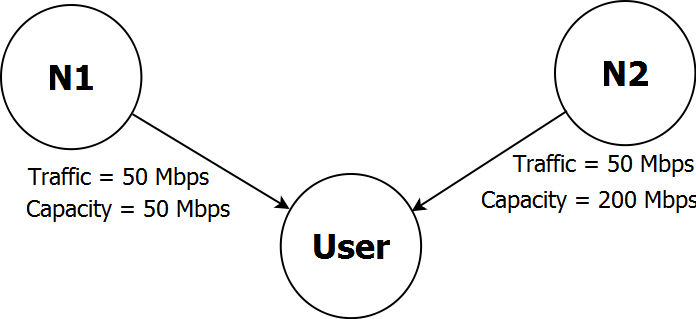
\includegraphics[scale=0.25]{final_images//Diagram1.png}}
%\subfigure[load = 2.0]{\label{fig:load-2}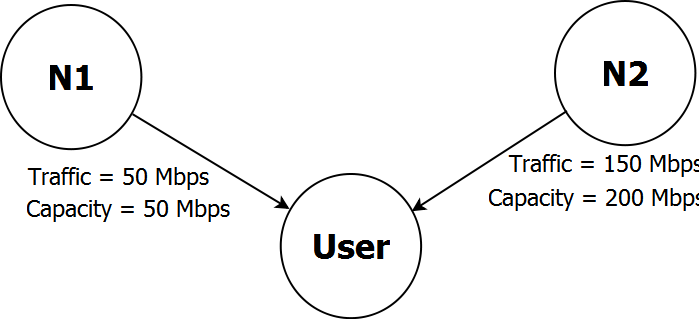
\includegraphics[scale=0.25]{final_images//Diagram2.png}}
%\subfigure[load = 3.0]{\label{fig:load-3}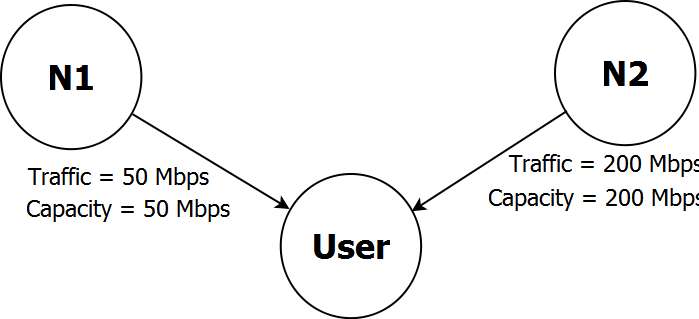
\includegraphics[scale=0.25]{final_images//Diagram3.png}}
%\end{center}
%\caption{Location diversity can change the traffic matrix}
%\label{fig:mlu_toy}
%\end{figure}
%

%\textbf{ but this does not hold with adaptation}

%Unfortunately, MLU is not a meaningful metric of capacity when application adaptation due to location diversity can change the traffic matrix itself. To appreciate this point, consider the example shown in Figure \ref{fig:mlu_toy}. Node 1 has a demand of 100 Mbps for content that can be fetched from either of nodes 2 or 3. Suppose node 1 splits the demand equally between the two locations, thereby resulting in an MLU of 1 by saturating the left link. Note that all TE schemes will result in the same routing as there is at most one route between each pair of nodes. Now suppose the demand at node 1 doubles to 200 Mbps. Node 1 can still satisfy its demand by fetching 50 Mbps and 150 Mbps along the left and right links respectively. Note that the MLU remains unchanged at 1 even though the demand has doubled. Furthermore, the doubling of demand does not simply scale the traffic matrix entries linearly, but instead changes them based on application behavior (e.g., based on how parallel TCP splits traffic across the two download locations). In general, it is difficult to predict how application behavior might change the traffic matrix as demand increases, as that change depends upon the underlying routing that in turn depends upon the original matrix. Indeed, even if the demand remains unchanged, the mere act of engineering routes (not observable in Figure \ref{fig:mlu_toy} as there is no route diversity) can change the traffic matrix when applications have location diversity.

%It is difficult to predict SPF using MLU if the network has application adaptation. This is because application adaptation can change the traffic matrix.  We show it using an example.  In Figure~\ref{fig:load-1} at load = 1.0 User node has a demand for 100Mbps traffic and it splits its demand equally and downloads 50Mbps each from N1 and N2. In Figure~\ref{fig:load-2}) at load = 2.0, the User node can still serve its demand by downloading 50Mbps from N1 and 150Mbps from N2. The metric MLU is not relevant in both cases since the application can change the traffic matrix to serve its demand. Empirically too we observed that the MLU value did not show a clear demarcation at a load where network is below capacity and the load where network is above capacity.

%\subsection{An empirical capacity measure}

%\textbf{proposing a new metric}

%We propose a new metric, {\em surge protection factor} (SPF), to quantify the capacity achieved by a TE scheme with respect to a traffic matrix. Let $E$ denote a TE scheme, $M$ the demand\tbd{Need to clarify that demand is a ``content matrix''.}, and MLU$(E,M)$ the MLU achieved by $E$ given $M$. When there is no location diversity, SPF$(E,M)$ is simply the inverse of MLU$(E,M)$, i.e., the factor of increase in the demand that can be satisfied. However, when there is location diversity, SPF$(E,M)$ is an {\em empirical} measure of the factor of increase in demand that can be satisfied, and is computed as follows. Let $kM$ denote the demand that scales each entry in $M$ by a factor $k>1$. Then, SPF$(E,M)$ is defined as the largest $k$ such that the routing computed by $E$ can satisfy the demand $kM$.

\subsection{Empirically measuring capacity}
Our metric of capacity is the SPF, i.e., the maximum surge in demand that can be satisfied (as  defined formally in Section \ref{sec:SPFdefinition}). Analytically determining whether an engineering scheme can satisfy a projected demand is difficult as it requires us to accurately model application adaptation  to location diversity, so the SPF must be determined empirically. In our experiments, we use a metric called {\em maximum input output difference} (or \maxiodiff) to determine whether a given demand can be satisfied. For each node, the {\em input} is the total traffic (bits/sec) requested by that node, while the {\em output} is the total traffic received by that node. \maxiodiff\ is defined as the maximum across all nodes of the relative difference between the input and output, i.e., {\em (input - output)/input}. If \maxiodiff\ is measured to be less than 0.1, then the demand is considered as satisfiable. We allow for a small difference in order to account for measurement error as well as to account for bursts in demand over the measurement duration.

%
%\begin{figure}
%\vspace{-0.1in}
%  \begin{center}
%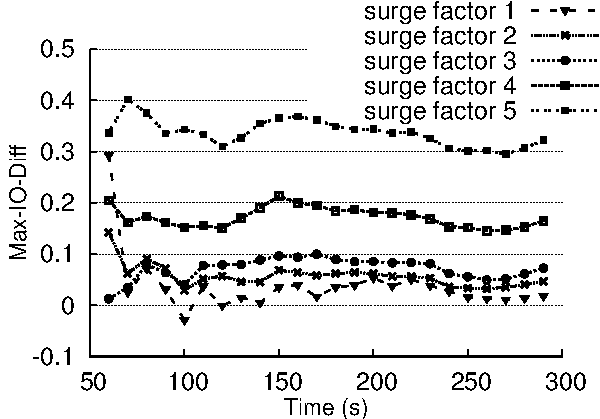
\includegraphics[scale=0.55]{final_images/G5_IOdiff/i_o_diff_plot.pdf}
%  \end{center}
%  \caption{Profile of \maxiodiff{} at increasing surge factors for a Geant TM}
%  \label{fig:input_output_diff}
%\end{figure}
%
%  \begin{figure}
% \begin{center}
%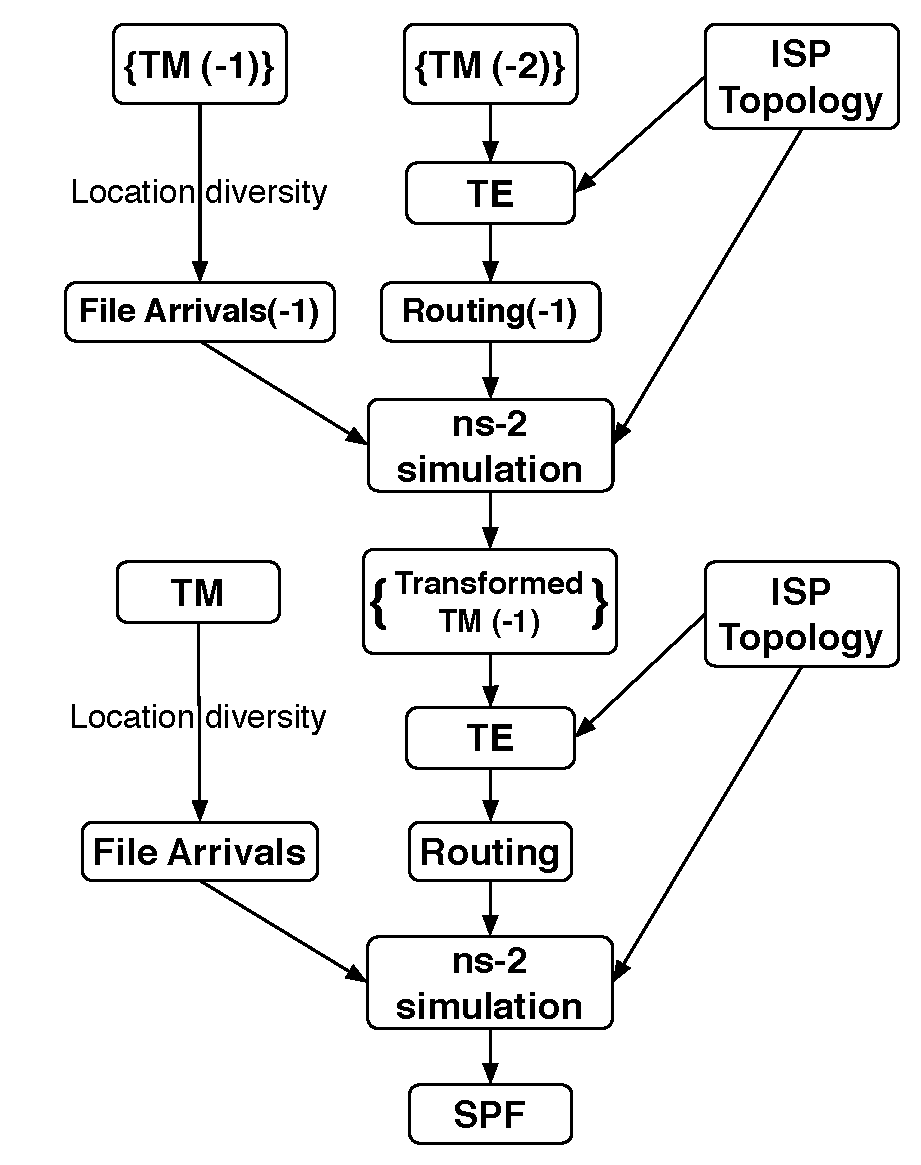
\includegraphics[scale=0.4]{final_images/Simulation2.pdf}
%\caption{Block diagram of experiment process with location diversity}
% \end{center}
% \label{fig:simulation2}
% \end{figure}


%\tbd{The reader may wonder why we could not have used the empirically measured MLU instead of \maxiodiff\ above, i.e., to consider a demand as satisfied if the measured MLU is less than 1 instead of of \maxiodiff\ is less than 0.1.}


% There are a couple reasons for this. First, the empirically measured MLU can never exceed 1, so the cutoff has to be a value somewhat less than 1. Second, as in the previous section, we find MLU to be a poor predictor of application performance, e.g., a higher MLU may result in equivalent or better application performance. This disparity between application performance and MLU only exacerbates under location diversity. We were unable to determine an empirical cutoff for the MLU that clearly delineates workloads that can be satisfied from those that can not.


%We propose a new metric to answer the above question - \emph{the maximum relative input-output difference}. Input for a node is the total traffic requested by users at the node. Output for a node is the total traffic received by users at the node. For each node with non-zero input, we compute its relative input-output difference as follows : Relative Input-Output Difference = (Input - Output)/Input. If input is zero for a node, we define its relative input-output difference as zero. Our metric is the maximum relative input-output difference over all nodes in the network. We will refer to this metric as \emph{\maxiodiff{}} from now on. 

%\textbf{use diagram to explain why it works}

%We illustrate this metric using the topology in Figure~\ref{fig:mlu_toy} again.  At load = 2.0 in Figure~\ref{fig:load-2} node User has demand for 200Mbps traffic. This demand is served by N1 sending 50Mbps and N2 150Mbps. In this case, the network has the capacity to serve demand and the \maxiodiff{} of the network is zero. At load = 3.0 in Figure~\ref{fig:load-3} traffic demand at User is 300Mbps and the total capacity of incoming links in 250Mbps. The network does not have capacity to serve this demand and the \maxiodiff{} is 50Mbps/300Mbps = 16.67\%. A positive value of \maxiodiff{} implies network does not have capacity for the demand.

%\textbf{more general than MLU}


%\textbf{Claim about metric}
%We make the following claim about this metric: 

%\emph{For a static traffic demand in the network, if \maxiodiff{} is p\%  (p $>$ 0), then network has capacity for p\% lesser traffic demand. It follows that if p = 0, network has capacity for the current demand.}

% If the network has capacity to serve the demand then p $=$ 0.
%We present a formal proof of the above claim in the Section~\ref{sec:appendix}.

%\textbf{How we measure it experimentally}

%We measure \maxiodiff{} in ns-2 simulations as follows: For each node, input is the sum of sizes of all files (measured in bytes) requested for download at the node. The output at the node is sum of the number of bytes of all files downloaded at the node. The difference is equal to the size of unfinished file downloads at the node. The relative input output difference for a node is the ratio of unfinished file downloads to the input and the \maxiodiff{} of the network is maximum relative input-output difference over all the nodes.

%\textbf{graph generated from simulation}


\maxiodiff\ helps clearly distinguish workloads that can be satisfied. For example, in Figure~\ref{fig:input_output_diff}, we show a \maxiodiff{} profile for five experiments at surge factors of 1, 2, 3, 4 and 5 for a Geant TM with \invcap{} routing.  The graph shows the \maxiodiff{} measured at intervals of 10 seconds throughout the simulation.
%The X-axis shows the progress of simulation. 
We ignore the first 50 seconds of simulation as the input significantly exceeds output at the start of simulation. We observe that beyond the initial period of fluctuation, \maxiodiff\ is relatively stable and below 0.1 for surge factors 1--3 that can be satisfied, but significantly higher for surge factors 4 and 5 that can not be satisfied.
%\tbd{Will it be helpful to show a graph for why MLU does not delineate the capacity point well?}.


\begin{figure*}
\begin{minipage}{0.45\textwidth}
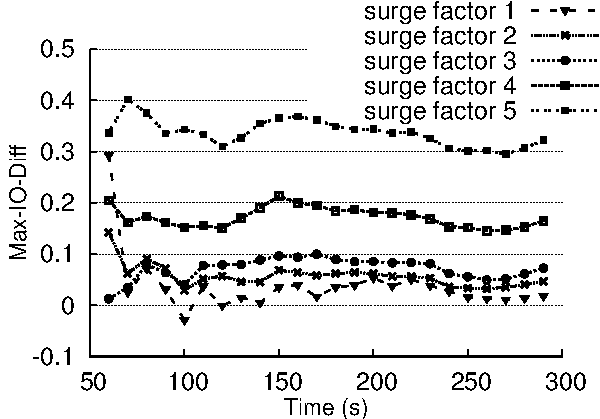
\includegraphics[scale=0.55]{final_images/G5_IOdiff/i_o_diff_plot.pdf}
  \caption{Profile of \maxiodiff{} at increasing surge factors for a Geant TM}
  \label{fig:input_output_diff}
\end{minipage}
\hspace{1cm}
\begin{minipage}{0.45\textwidth}
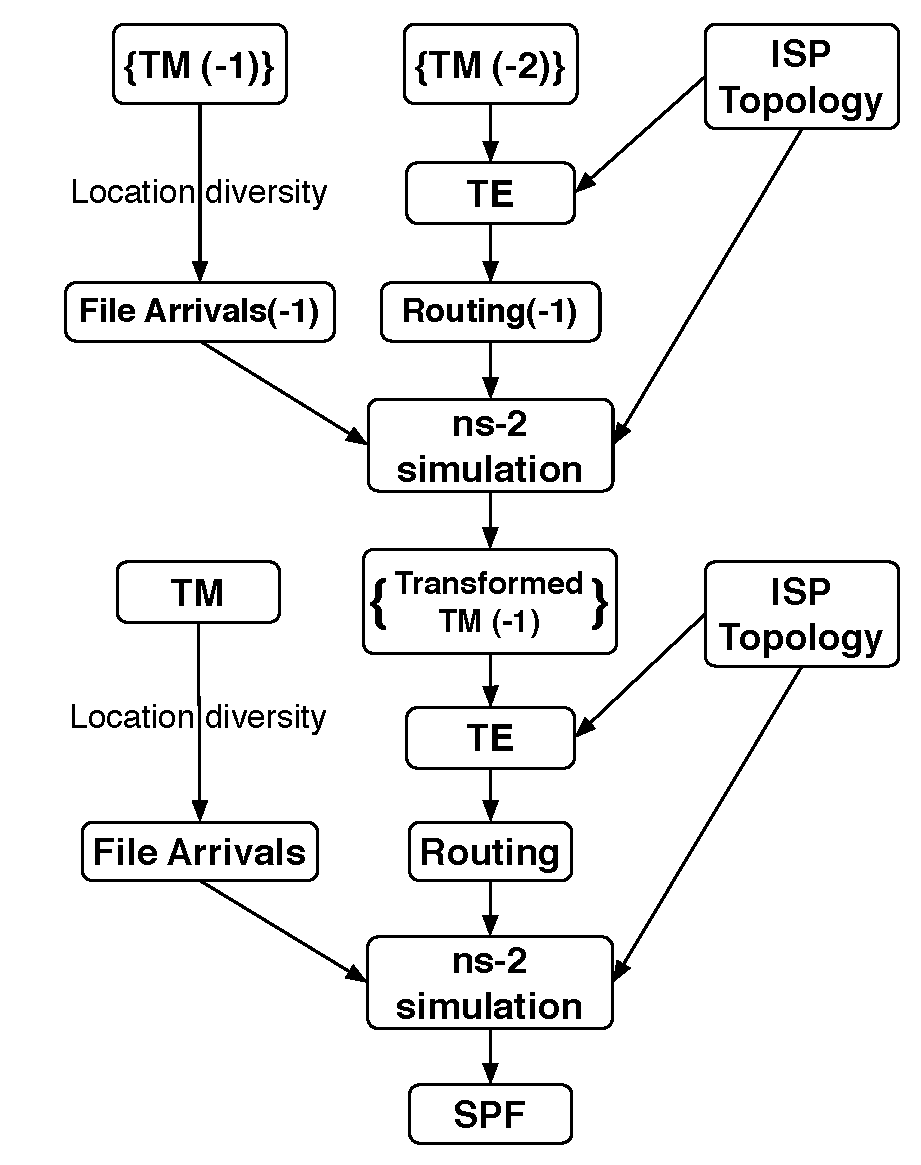
\includegraphics[scale=0.4]{final_images/Simulation2.pdf}
\caption{Block diagram of experiment process with location diversity}
 \label{fig:simulation2}
\end{minipage}
\end{figure*}


%Initial values vary significantly, but later the values vary within a range of a few percent and we infer that the \maxiodiff{} of the network lies in this range.

%
%\begin{figure}[t]
%  \begin{center}
%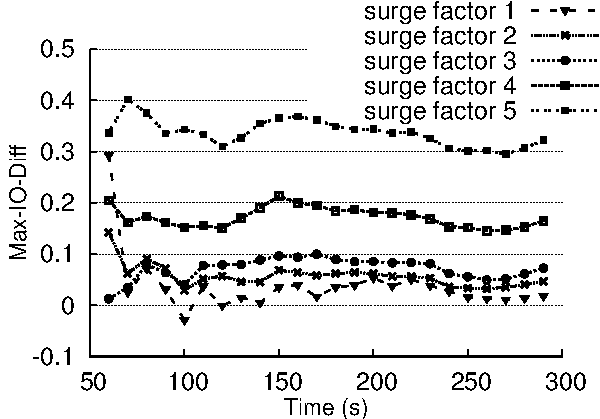
\includegraphics[scale=0.4]{final_images/G5_IOdiff/i_o_diff_plot.pdf}
%  \end{center}
%  \caption{Profile of \maxiodiff{} at increasing loads for a Geant TM and \invcap{} routing}
%  \label{fig:input_output_diff}
%\end{figure}

%\textbf{accommodating experimental errors}

%To decide if a network is has capacity for a given load, we need to accommodate two experimental artifacts: (1) As Figure~\ref{fig:input_output_diff} shows, the \maxiodiff{} varies within a few percent. Therefore, we take the average of 10 values of  \maxiodiff{} measured in the last 100s of simulation. (2) Experimentally, we observe that the  \maxiodiff{} is a small positive fraction even when the network has capacity. This is expected since we run our simulations for a short duration and some files have zero or very small download rates in our simulation. (This is explained in Section~\ref{sec:app_performance}). To account for it, we decide that the network has capacity at a given load if its \maxiodiff{} is less than 10\%. A 10\% error value in our simulation implies we can over predict the SPF of a network by at most 10\%. If we predict that the network has the capacity at load $x$ and $C$ is the SPF of the network, then $x < 1.1 C$.

%The average traffic demand for our simulation is static, therefore we can apply our claim stated above. According to our claim,  a 10\% difference in \maxiodiff{} implies that the network has is below capacity for a 10\% lesser demand.  

\subsection{Simulating location diversity}
\label{sec:ns2-multisource}

%An application can leverage location diversity in multiple ways. It can download in parallel from all locations or  download from the location which has the best performance (throughput/delay). Among these, we experiment with parallel downloads to model application adaptation. In our simulation, each file download is started simultaneously from all locations and file download finishes when total number of bytes downloaded from all locations equals the file size.

 
%\begin{figure}[tbh]
%  \begin{center}
%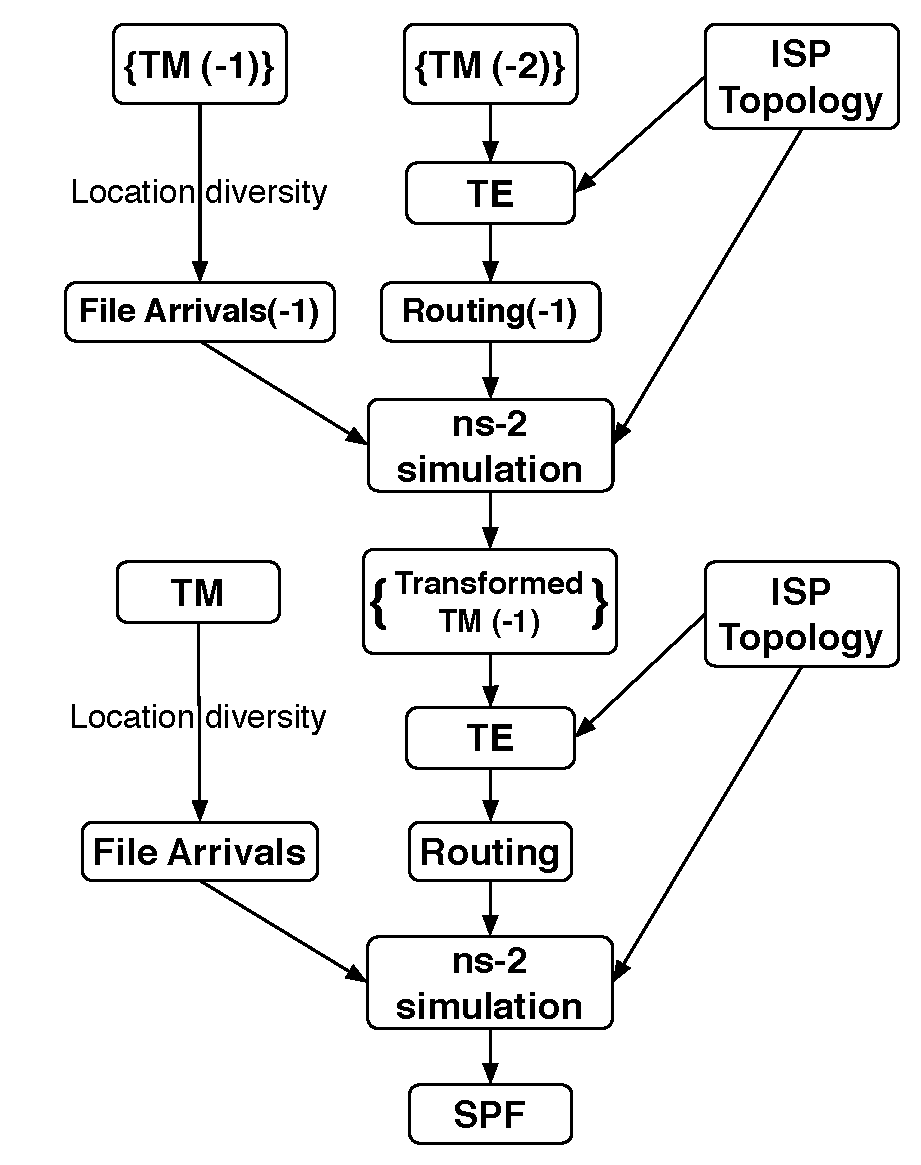
\includegraphics[scale=0.43]{final_images/Simulation2.pdf}
% \end{center}
%\vspace{-0.1in}
%	  \caption{Block diagram of experiment process with location diversity}
%  \label{fig:simulation2}
%\end{figure}

Figure~\ref{fig:simulation2} illustrates the experimental process with location diversity. The lower half  is similar to Figure~\ref{fig:simulation1} with two differences. First, to incorporate location diversity, we modify the procedure to transform {\em TM} to {\em File Arrivals} as follows. As in Section~\ref{sec:exp_setup}, we first transform PoP-to-PoP entries in {\em TM} to a sequence of file download requests. However, instead of downloading each file from just that one location, $k$-1  additional randomly chosen source locations are introduced so as to emulate a location diversity of $k$.  The file is downloaded in parallel from all $k$ locations using parallel TCPs. The download is considered complete when the total bytes downloaded across all $k$ locations equals the size of the file.

%except for the block \textsl{TM(-1)} that is replaced by \textsl{Transformed TM(-1)} in Figure~\ref{fig:simulation2}. The upper half of Figure~\ref{fig:simulation2} describes how \textsl{Transformed TM(-1)} is obtained from  \textsl{TM(-1)}.

%Another change which is not visible in the block diagram is the process of translating from \textsl{TM} to \textsl{File Arrivals}. This process is modified to incorporate the effect of location diversity. First we derive a sequence of  \textsl{File Arrivals} from  \textsl{TM} as described in Section~\ref{sec:exp_setup}. Then, we add ($k$ - 1) new locations, chosen randomly,  in addition to the original location from which each file can be downloaded.  $k$ is a location diversity parameter. Each file download initiates parallel TCP connections to the $k$ chosen locations in the network. A download is considered as completed when the total number of bytes download from all $k$ connections equals the size of the file.

Second, application adaptation to location diversity changes the input to {\em TE} as indicated by the block \textsl{Transformed TM(-1)} that is  obtained as follows. Let \textsl{TM(-1)} and \textsl{TM(-2)} respectively denote the (set of) matrix(ces) in the last and last-to-last epochs. Recall that {\em TE} determines the length of the epoch (0 for \opt, 3 hours for \optwt\ and \mplsavg\, and a day for \cope). \textsl{Transformed TM(-1)} is generated by the top simulation that takes as input the file arrivals obtained from \textsl{TM(-1)} and {\em Routing (-1)}. The latter is obtained by applying {\em TE} to \textsl{TM(-2)} in the previous epoch. This two-step simulation is intended to approximate the interaction of TE and application adaptation to location diversity that changes the TM. 

%the epoch length is determined by {\em TE} (e.g., \textsl{TM(-1)} is identical to {\em TM} for \opt\ but denotes the set of matrices in the most recent 3-hour ) The upper level simulation transforms 

%The need for \textsl{Transformed TM(-1)} arises because application adaptation to location diversity can change the traffic matrix.  \textsl{Transformed TM(-1)} is our estimate of the matrix resulting from the change in the matrix/matrices in the set \textsl{TM(-1)}. Note that \textsl{TM(-1)} is the either the current traffic matrix (for \opt) or the set of matrices from the previous  traffic engineering epoch (for other schemes). Using a ns-2 simulation, we simulate application adaptation for each matrix in \textsl{TM(-1)} and measure the resulting traffic matrix at the end of experiment.  The resulting set of matrices is \textsl{Transformed TM(-1)}.

%We do the simulation as follows (refer to Figure~\ref{fig:simulation2}): (1) Translate a matrix in \textsl{TM(-1)} to \textsl{File Arrivals} as described in the previous paragraph (2) Run \textsl{TE} algorithm to compute routing based on matrices in \textsl{TM(-2)}. Similar to \textsl{TM(-1)}, \textsl{TM(-2)} is either the current matrix (for \opt) or a set of matrices from the epoch \emph{before} the previous traffic engineering epoch (for other schemes). (3) Run \textsl{ns-2 simulation} using \textsl{File Arrivals}, \textsl{Routing} and \textsl{ISP Topology}. Finally, we measure the resulting traffic matrix.



%We start with a set of periodically logged traffic matrices from real ISPs in our dataset. Let $M_1, M_2,\cdots$ denote a sequence of such matrices and $E$ a TE scheme. As in the previous section, we translate each matrix $M_i$ to a file request arrival process. However, instead of downloading each file from just one location, we add $k-1$  randomly chosen source locations  from which the file is downloaded in parallel. The routes from the $k$ source locations to the sink are computed by applying $E$ to $M_i$. As a result of parallel downloads, each matrix $M_i$ will have changed, say, to a new matrix $N_i$.

%In the second step, we recompute routes by applying $E$ periodically to the appropriately time-averaged matrix. For example, if $E$ is \opt, we recompute routes periodically (once every 5, 15, or 60 minutes depending upon our ISP dataset) based on $N_i$ at that time instant. For \optwt, we recompute routes once every 3 hours using a matrix that is the average of the matrices in the past 3 hours, and so on. %We note that the recomputed routes and parallel downloads may again change $N_i$, resulting in a different MLU than engineered for, but this mismatch between engineering and application adaptation to location diversity is exactly what we seek to capture in our simulations.



%We note that an alternate form of location diversity is to download content from a single ``best'' location. However, we chose parallel downloads as they are simple, do not require any additional infrastructure for server selection, and are in widespread use in P2P systems today. 

%We define a location diversity parameter '$k$' - the number of locations content is present in the network.

%Experiments in this section include two types of ns-2 simulations : (1) Users download files from one source node only ($k = 1$) (2) Users download files in parallel from multiple locations ($k > 1$). We have already described our experiment with single location downloads. Our experiment with multiple locations is a two-step process which we explain next.





%We need two steps of simulation because application adaptation changes the traffic matrix. After the first step of simulation, we measure the adapted traffic matrix. In the next step, we compute routing based on the adapted traffic matrix.

%\subsubsection{Simulating a Traffic Matrix with Location Diversity}
%\textbf{why 1 ns-2 simulation is not accurate }
%Earlier while simulating single location download, we generated a file arrival sequence from the traffic matrix given. Next, we computed the routing based on current traffic matrix or a set of previous traffic matrices depending on routing. Then we simulated the arrival sequence in network with the given routing.

%A simple way to simulate a traffic matrix with location diversity is as follows: We compute the routing and we generate a file arrival sequence from the traffic matrix identical to single location download. But we choose (k - 1) additional source locations for each file. Then, we simulate parallel download of each file from k locations.

%But such a simulation does not ensure a fair comparison of TE schemes. The reason is that the traffic matrix resulting from parallel download simulation is likely to be very different from the original traffic matrix. But, the TE scheme had computed the routing assuming the original traffic matrix.

%Let S be the original set of TMs in our dataset and T $\in$ S be the TM we want to simulate with location diversity. The first step computes a file arrival process for this TM. The second step computes routing for this TM.

%\emph{First Step:} We compute a file arrival sequence for T identical to single location download. But we choose ($k - 1$) additional source locations for each file. Each file will be downloaded in parallel from these $k$ locations during the simulation. Since we split traffic among $k$ locations for each file download, it is expected that TM will be changed significantly during simultation.

%\emph{Second Step: } Computing a routing for T is difficult since we do not yet know the changed traffic matrix that will result from simulation. Routing for T may depend on T or a subset of other TMs in S as well. For example, \optwt{} computes routing on the average of past 3 hour TMs. These other TMs would also change due to location diversity which makes it more difficult to compute routing for T. We work around this problem as follows:  Through ns-2 simulations, we obtain a new set of TMs S' from set S which have changed due to location diversity in the network. We compute a routing for T based on the new set of TMs S'.

%We obtain the TMs in set S' as follows: For each TM in set S, we compute the routing and we generate a file arrival sequence from the traffic matrix identical to single location download. But we choose ($k - 1$) additional source locations for each file. Then, we simulate parallel download of each file from $k$ locations and measure the new traffic matrix. 


%\textbf{optimization}

%We optimize the simulation process by only computing those matrices in set S' which determine the routing for TM T. We compute the TMs depending on the TE scheme: \opt{} computes routing based on current TM, hence we only compute the adapted version of current TM; \optwt{} and  \mplsavg{} use the average of past 3 hour TMs, hence we average the TMs of past 3 hours from set S and compute its adapted version; \cope{} computes routing using all matrices from previous day but we use a random selection of 4TMs from previous day and compute routing using the adapted versions of these TMs;  the routing for \invcap{} is fixed.

\subsection{Experimental procedure}

%\textbf{experimental data and parameters}

The experiments to determine SPF involve a computationally intensive search across many different surge factors for each matrix. Furthermore, at high surge factors, the number of ns-2 data structures required to simulate ongoing parallel TCP connections becomes prohibitively high. So for computational tractability, we selected 4 matrices each from one day of data of each ISP. The matrices were selected randomly, one from each 6-hour duration during the day.  For each matrix and each engineering scheme, we conduct an experiment at each value of the surge factor starting from 1 in increments of 0.25 until the capacity point is reached, i.e., the \maxiodiff\ value exceeds 0.1. Each experiment is run until the \maxiodiff\ value stabilizes or 300 seconds, whichever is greater. 

%We selected only 4 TMs since we did 50-100 simulations with each TM. Experiments in this section were more computationally demanding since we experimented with higher loads which increased the number of file downloads we simulated and each file download used multiple TCP connections which increased the number of ns-2 data structures. Each experiment was run for 300s duration, but in some cases we did 500s experiments if the \maxiodiff{} didn't reached a stable value in 300s. Similar to Figure~\ref{fig:input_output_diff}, we compute \maxiodiff{} every 10 seconds.

%\textbf{how we calculate capacity}

%We calculated the SPF value by simulating a traffic matrix at increasing loads. We started with original TM (load 1), increased load by 0.25 at every step and checked if the network has capacity at that load. We select the highest load at which network had capacity as the SPF value.

%\textbf{upper and lower bounds}

%Our experimental procedure gives us following upper and lower bounds on the actual capacity of the network. If $x$ is the capacity we 
%measure and $C$ is the actual capacity, then : (1) $C < x + 0.25$. This is because we experiment with loads at intervals of 0.25. (2) We have already shown that $x < 1.1C $. Combining the upper and lower bounds for our experimental error \[x/1.1 < C < x + 0.25\]

%We use this equation to calculate confidence intervals for our results.

%% graphs for capacity using linear program
%\begin{figure}[t] \begin{center} 
%\subfigure[Abilene Optimal]{\label{fig:edge-a}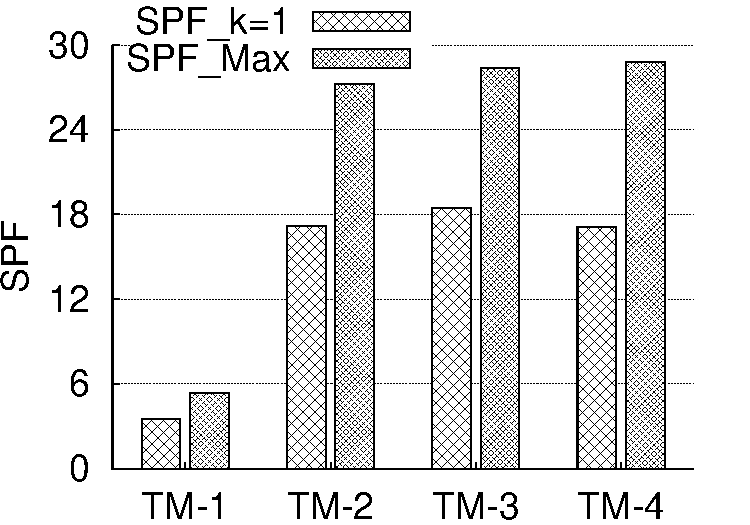
\includegraphics[scale=0.33]{final_images/G9_optcapacity/Abilene_opt_hist_plot.pdf}}
%\subfigure[Abilene InvCap]{\label{fig:edge-a}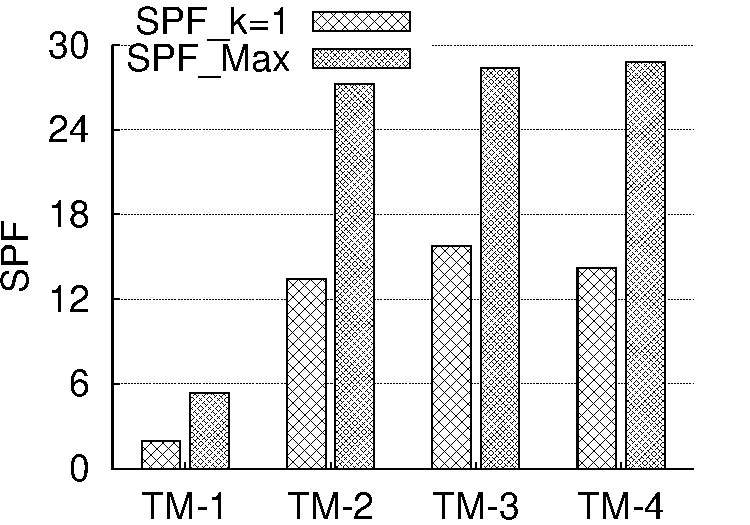
\includegraphics[scale=0.33]{final_images/G9_optcapacity/Abilene_inv_hist_plot.pdf}}
% \subfigure[Geant Optimal]{\label{fig:edge-b}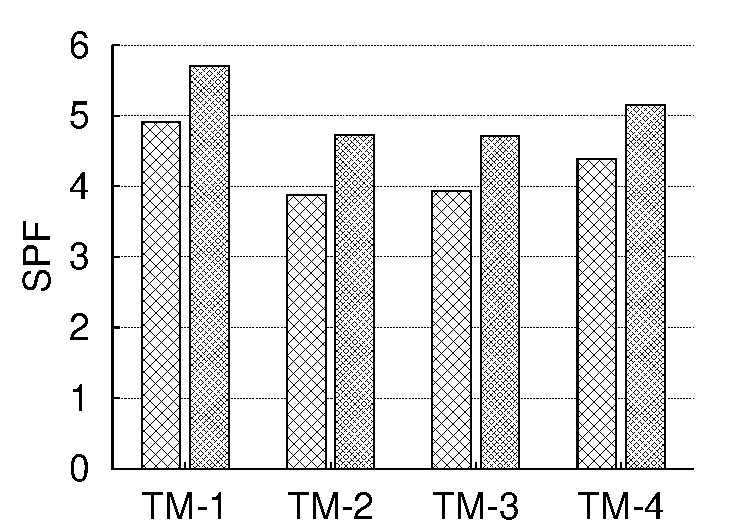
\includegraphics[scale=0.33]{final_images/G9_optcapacity/Geant_opt_hist_plot.pdf}}
% \subfigure[Geant InvCap]{\label{fig:edge-b}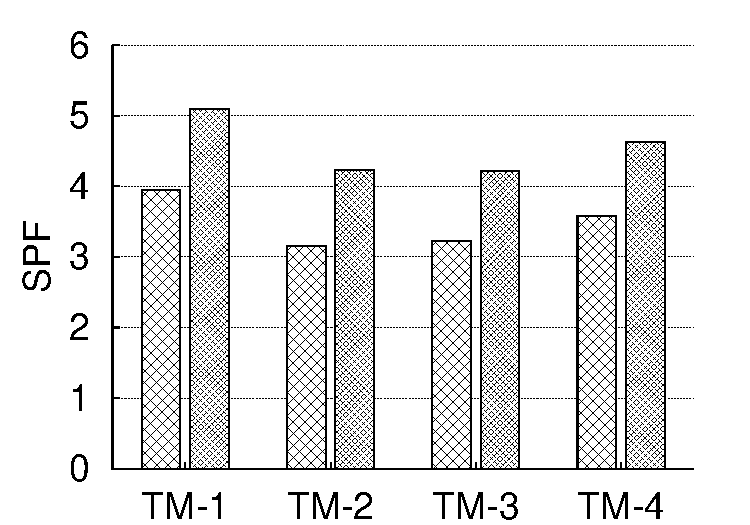
\includegraphics[scale=0.33]{final_images/G9_optcapacity/Geant_inv__hist_plot.pdf}}
%\subfigure[US-ISP Optimal]{\label{fig:edge-c}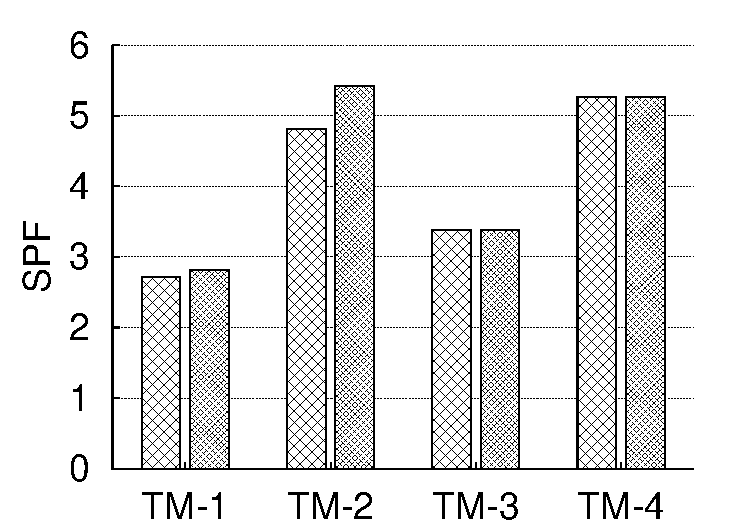
\includegraphics[scale=0.33]{final_images/G9_optcapacity/USISP_opt_hist_plot.pdf}}  
%\subfigure[US-ISP InvCap]{\label{fig:edge-c}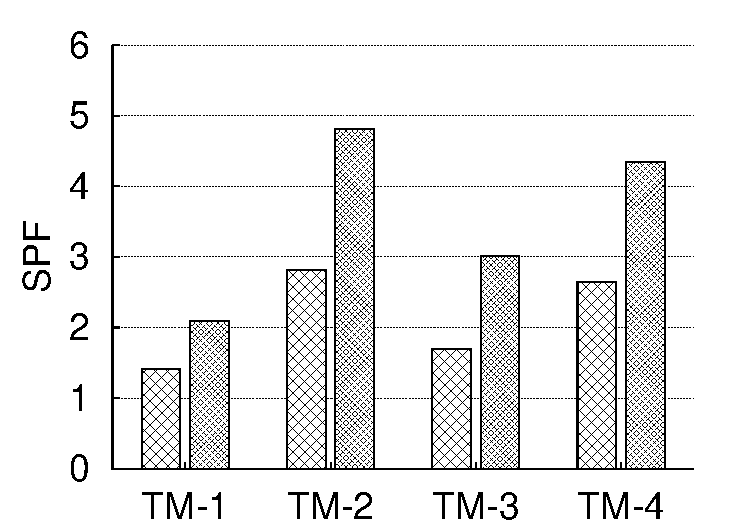
\includegraphics[scale=0.33]{final_images/G9_optcapacity/USISP_inv_hist_plot.pdf}}  
%\end{center}\caption{\label{fig:capacity_opt} Maximum SPF for \opt{} and \invcap{} routing calculated using linear program.}
%\vspace{-0.2in}
%\end{figure}


% graphs for capacity using ns-2 simulations


\begin{figure*}[t] \begin{center} 
\subfigure{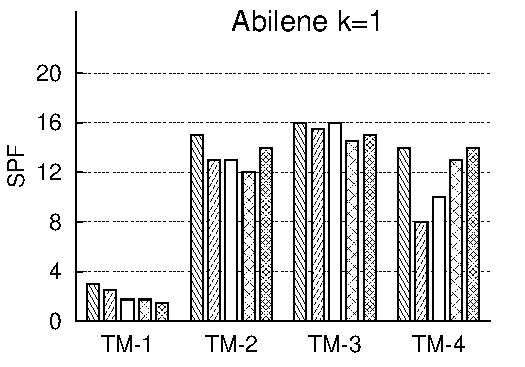
\includegraphics[scale=0.5]{final_images/G6_capacity/Abilene/k1_hist_plot.pdf}}
\subfigure{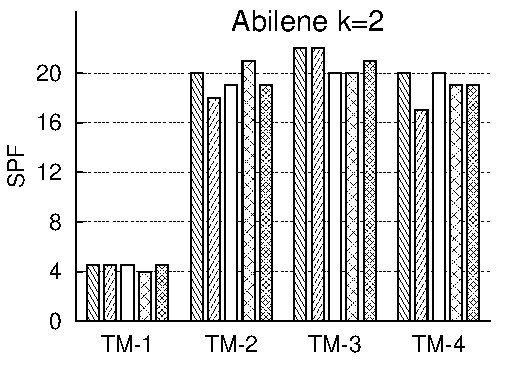
\includegraphics[scale=0.5]{final_images/G6_capacity/Abilene/k2_hist_plot.pdf}}
\subfigure{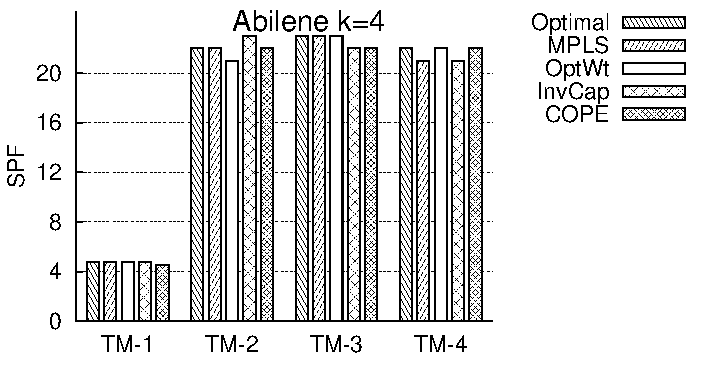
\includegraphics[scale=0.5]{final_images/G6_capacity/Abilene/k4_hist_plot.pdf}}
 \subfigure{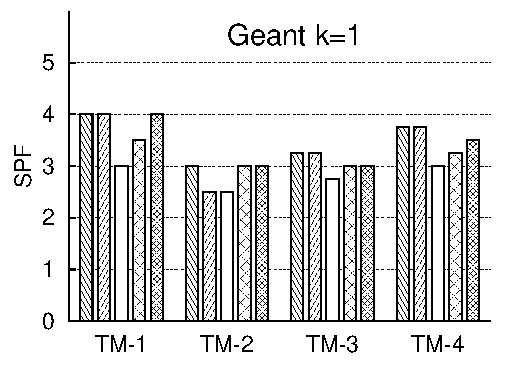
\includegraphics[scale=0.5]{final_images/G6_capacity/Geant/k1_hist_plot.pdf}}
 \subfigure{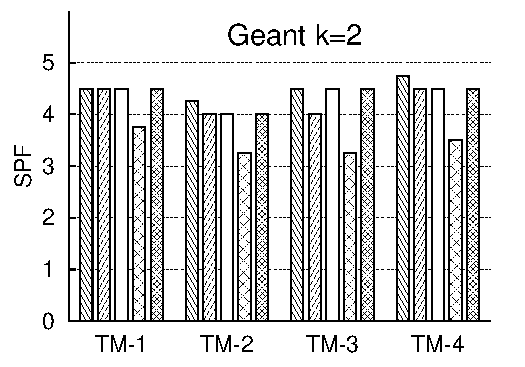
\includegraphics[scale=0.5]{final_images/G6_capacity/Geant/k2_hist_plot.pdf}}
 \subfigure{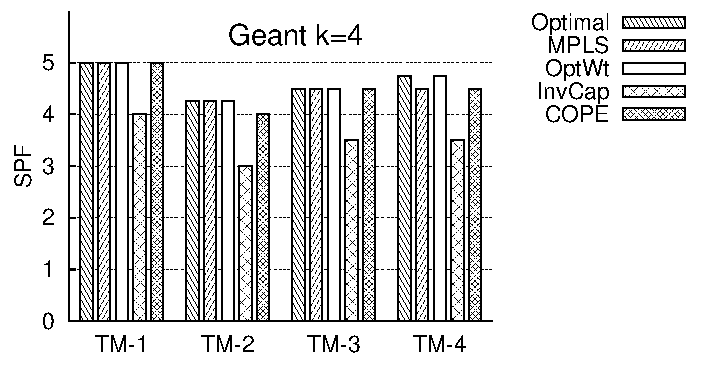
\includegraphics[scale=0.5]{final_images/G6_capacity/Geant/k4_hist_plot.pdf}}
\subfigure{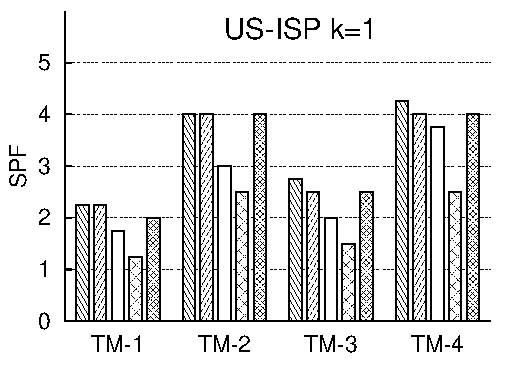
\includegraphics[scale=0.5]{final_images/G6_capacity/USISP/k1_hist_plot.pdf}}
\subfigure{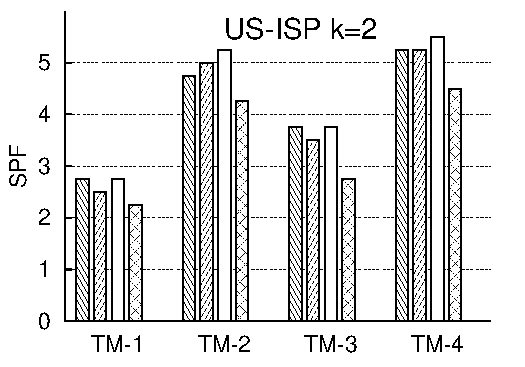
\includegraphics[scale=0.5]{final_images/G6_capacity/USISP/k2_hist_plot.pdf}}
\subfigure{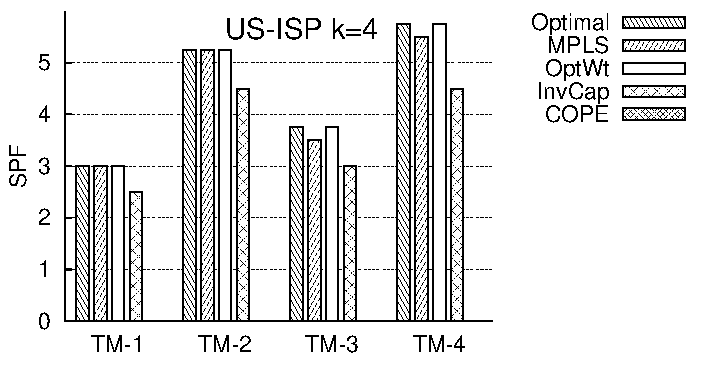
\includegraphics[scale=0.5]{final_images/G6_capacity/USISP/k4_hist_plot.pdf}}
 \end{center}
\caption{\label{fig:capacity_diversity} Comparison of SPF among TE schemes for different levels of location diversity; SPF values are obtained using ns-2 simulations }
\vspace{-0.2in}
\end{figure*}

\subsection{Capacity increase with location diversity}
%
%We first present our results for the maximum capacity increase as calculated by the linear program in technical report \cite{TR}, and then as measured experimentally.

%\subsubsection{Theoretical capacity increase with location diversity}

%%\textbf{explaining the graph presented}

%In Figure~\ref{fig:capacity_opt}, we present the results for the maximum SPF using \opt{} and \invcap{} routing for the selected TMs. For each TM, the left bar shows the SPF  without location diversity ($k = 1$) and the right bar shows the SPF when a node can obtain content from all nodes in the network except itself ($k = n - 1$, $n  =$ number of nodes). Note that the later case is the maximum SPF which can be achieved with location diversity.

%%While \opt{} has the freedom to split flows arbitrarily among multiple locations and  to choose any routing, \invcap{} can split flows arbitrarily among multiple locations but is restricted to use the default shortest path routing. 

%%\textf{How linear program works}
%%The linear program works as follows: For every node pair ($i$,$j$) where $i$ is the source and $j$ is the destination, the original flow without location diversity is equal to the traffic matrix entry $f_{i,j}$.  We add $(k - 1)$ new sources randomly for this flow and solve the linear program which optimizes the MLU. If the optimal MLU obtained from the linear program is $\alpha$, then the capacity of the network is $1/\alpha$.  We increase the value of $k$ from 1 to $(n-1)$ where $n$ is the number of nodes in the network. The optimal routing can be achieved using $m$ locations, where $m \leq (n-1)$. 

%%\textbf{what is the capacity increase}

%The capacity increase in the network for \opt{} is  1.6$\times$ for Abilene,  1.2$\times$ for Geant and less than 1.1$\times$ for US-ISP topology. The capacity increase for \invcap{} is approx 2.1$\times$ for Abilene, 1.3$\times$ for Geant topology and 1.5$\times$ for US-ISP topology.  Clearly location diversity increases the capacity both for \opt{} and \invcap{} but the increase depends on the ISP topology and traffic matrix. \invcap{} has less capacity than \opt{} even with location diversity but the relative difference between the two has diminished. This result shows that location diversity reduces the difference in capacity among TE schemes.

%

%%\textbf{only few locations get max capacity increase}

%While $(n-1)$ locations can certainly give the maximum SPF, we find only 2-4 locations can give the maximum SPF for most matrices both for \invcap{} and \opt{}). The reason is that the immediate links to some nodes often become the bottleneck first. As each node in these ISP topologies typically has on average only a few incoming links (3-4 links), even a small number of additional locations suffice to saturate all incoming links for the most loaded node in the network.
%%traffic equally on all incoming links in the network. %Thus the network achieves the optimal MLU routing only with a small degree of location diversity.

%%\textbf{summary sentence}

%%Results from linear program solutions show that location diversity not only increases the capacity of the network but also reduces the difference in capacity among TE schemes.

%\subsubsection{Capacity increase for location diversity using ns-2 simulations}

%\textbf{why LP is not practical?}

%The capacity increase calculated above using a linear program may not be achievable in practice. There are two reasons for this. First, users in a network may not split their flows optimally among multiple locations as in the linear program solution. Second, the routes computed using any realistic TE scheme would in general be different from the optimal routing computed above. Nevertheless, we find that location diversity increases the capacity significantly for all TE schemes.

In Figure~\ref{fig:capacity_diversity}, we present the SPF values obtained using ns-2 simulations for the selected TMs. We compared all TE schemes for three levels of location diversity: $k = 1, 2$ and $4$.  Note that we do not present the results for \cope{} for US-ISP (k =2 and k = 4), since the implementation of \cope{}'s algorithm failed to compute a feasible set of routes even after 12 hours of simulation time (1 million iterations)  after which we aborted the simulation. We have used authors' implementation of the algorithm and communication with them confirmed that indeed in some cases \cope{}'s implementation can take a long time to terminate. This happens in cases where barrier-crossover method to solve a linear program fails and \cope\ instead uses simplex method which is much slower.


The average capacity increase for \opt{} from $k = 1$ to $k = 4$ is 1.41$\times$ and from $k = 1$ to $k = 2$ is 1.31$\times$. \opt{} is the maximum SPF for a network with no location diversity ($k = 1$). This shows that a network with location diversity of $k = 4$ has 40\% greater capacity than a network with no location diversity. Even location diversity of $k = 2$ gives $75\%$ of capacity increase obtained from location diversity of $k = 4$. 

%
%
%  \begin{tabular}{ p{1.8cm} | p{0.4cm} | p{0.4cm} | p{0.4cm}  | p{0.4cm}  }
%\hline
%TE/\opt{}&  k=1& k=2 & k=4 \\ \hline
%\opt{}/\opt{} & 1 (1) & 1 (1)  & 1(1)   \\ 
%\mplsavg{}/ \opt{} & 0.89 () & 98 & 0.99 \\
%\optwt{}/\opt{} & 0.73 & 0.99 & 0.99 \\
%\invcap{}/\opt{} & 0.91 & 0.86 & 0.85  \\
%\cope{}/\opt{} & 0.91 & 0.99  & 0.98 \\  \hline
%  \end{tabular}
%

%\begin{figure*}[tbh]

%\begin{minipage}{2in}\footnotesize
%\begin{center}
%  \begin{tabular}{ p{1.8cm} | p{0.4cm} | p{0.4cm} | p{0.4cm}  }
%\hline
%TE/\opt{}&  k=1  & k=2 & k=4 \\ \hline
%\opt{}/\opt{} & 1 & 1 & 1 \\ 
%\mplsavg{}/ \opt{} & 0.89 & 98 & 0.99 \\
%\optwt{}/\opt{} & 0.73 & 0.99 & 0.99 \\
%\invcap{}/\opt{} & 0.91 & 0.86 & 0.85  \\
%\cope{}/\opt{} & 0.91 & 0.99  & 0.98 \\  \hline
%  \end{tabular}
%\vspace{0.2in}
%  \caption{Comparison of SPF values}
%\vspace{-0.3in}
%  \label{fig:cap_comparison}
%\end{center}
%\end{minipage}
%\hspace{0.5cm}
%\begin{minipage}{2in}
%  \begin{center}
%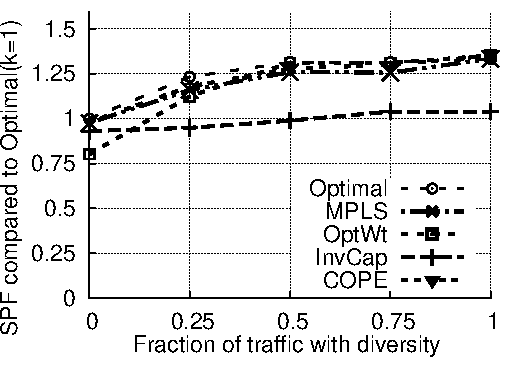
\includegraphics[scale=0.6]{final_images/G11_div_nodiv/Geant_k4/Geant_k4.pdf}
%  \end{center}
%  \caption{Effect of partial location diversity for Geant TMs.}
%  \label{fig:capacity_fraction_diversity}
%\end{minipage}
%\hspace{0.5cm}
%\begin{minipage}{2in}
%  \begin{center}
%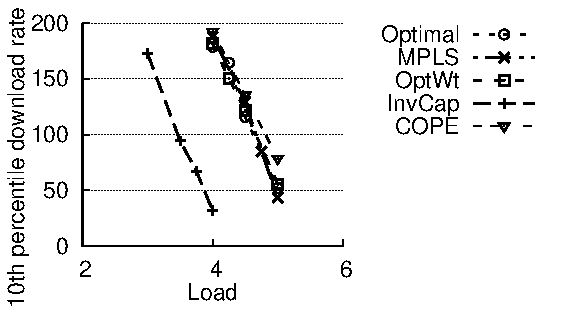
\includegraphics[scale=0.7]{final_images/Geant_TCP_points_plot.pdf}
%%\subfigure[UDP]{\label{fig:UDP_higher_loads}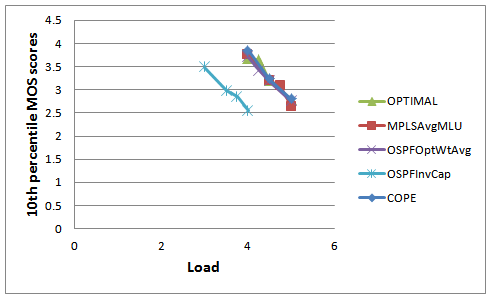
\includegraphics[scale=0.35]{final_images/UDP_higher_loads.png}}
%  \caption{TCP performance at increasing loads for Geant TM}
%\label{fig:TCP_higher_loads}
%  \end{center}
%%\label{fig:TCP_higher_loads}
%\end{minipage}
%\vspace{-0.2in}
%\end{figure*}




%\begin{figure}\footnotesize
%\begin{center}
%
%  \begin{tabular}{| l | c |  c | c |  c }
%\hline
%Routing / Routing &  k = 1  & k = 2 & k = 4 \\ \hline
%\opt{} / \opt{} & 1 & 1 & 1 \\ 
%\mplsavg{} / \opt{} & 0.89 & 98 & 0.99 \\
%\optwt{} / \opt{} & 0.73 & 0.99 & 0.99 \\
%\invcap{} / \opt{} & 0.91 & 0.86 & 0.85  \\
%\cope{} / \opt{} & 0.91 & 0.99  & 1.02 \\  \hline
%  \end{tabular}
%\vspace{0.2in}
%  \caption{Comparison of SPF values}
%\vspace{-0.3in}
%  \label{fig:cap_comparison}
%\end{center}
%\end{figure}

%\textbf{location diversity reduces TE differences}

%Over all TMs, \opt\ has 

%The maximum difference among \opt\ and other 


%Location diversity significantly reduces the difference in capacity among TE schemes. In fact, other TE schemes perform better than \opt\ in some cases. This is because location diversity changes the TM after optimal TE is implemented 
\begin{figure}\footnotesize
\begin{center}
  \begin{tabular}{ l | c | c | c  }
%  \begin{tabular}{ p{1.8cm} | p{0.4cm} | p{0.4cm} | p{0.4cm}  }
TE/\opt{}&  k=1  & k=2 & k=4 \\ \hline
\opt{}/\opt{} & 1 & 1 & 1 \\ 
\mplsavg{}/ \opt{} & 0.89 & 0.98 & 0.99 \\
\optwt{}/\opt{} & 0.73 & 0.99 & 0.99 \\
\invcap{}/\opt{} & 0.91 & 0.86 & 0.85  \\
\cope{}/\opt{} & 0.91 & 0.99  & 0.98 \\  
  \end{tabular}
  \caption{Comparison of SPF values}
  \label{fig:cap_comparison}
\end{center}
\end{figure}
Location diversity enables all TE schemes to achieve near-optimal capacity. In Figure~\ref{fig:cap_comparison} we compare the SPF of \opt{} to that of other TE schemes. The statistic presented is ratio of SPF of TE scheme to SPF  of \opt{} for the same level of location diversity averaged over all TMs. Except \invcap{}, all TE schemes have SPF within 2\% of \opt\ for $k= 4$ as well as $k = 2$. Figure \ref{fig:capacity_diversity} shows that with location diversity any TE scheme has at most 10\% capacity difference compared to \opt. On average \invcap{} has 15\% less capacity compared to \opt{} for a location diversity of  $k = 4$.  In the worst case \invcap\ achieves a capacity that is 30\% less than \opt\ (Figure \ref{fig:capacity_diversity}, Geant k = 2).

%\begin{figure}\footnotesize
%  \begin{tabular}{ p{1.8cm} | p{0.4cm} | p{0.4cm} | p{0.4cm}  }
%\hline
%TE/\opt{}&  k=1  & k=2 & k=4 \\ \hline
%\opt{}/\opt{} & 1 & 1 & 1 \\ 
%\mplsavg{}/ \opt{} & 0.89 & 0.98 & 0.99 \\
%\optwt{}/\opt{} & 0.73 & 0.99 & 0.99 \\
%\invcap{}/\opt{} & 0.91 & 0.86 & 0.85  \\
%\cope{}/\opt{} & 0.91 & 0.99  & 0.98 \\  \hline
%  \end{tabular}
%  \caption{Comparison of SPF values}
%  \label{fig:cap_comparison}
%\end{figure}

The above result calls into question the usefulness of online TE schemes. In today's Internet, offline TE schemes such as \optwt{} or \mplsavg{} are commonly used. It is believed that these schemes are sub-optimal and online TE schemes (e.g., TeXCP, MATE etc.) can achieve near-optimal capacity.  However, our results suggest that application adaptation to location diversity results in near-optimal SPF for all TE schemes.  Even the shortest-path routing scheme, \optwt{}, achieves the same SPF as TE schemes employing MPLS for flow splitting.



%In contrast, without location diversity \opt{} has upto 2$\times$ higher capacity than \invcap{} for some TMs.

%In comparison without any location diversity, \opt\ has up to 2$\times$ more capacity than \invcap\ for some traffic matrices. 


%While \invcap\ reduces its relative capacity difference compared to \opt\, it still remains sub-optimal.
%Based on this, we conclude that although application adaptation significantly undermines the value of traffic engineering, it does not obviate it completely.

%On average \invcap{} has 85\% capacity compared to \opt{} even for a location diversity of $k = 4$.  \invcap{} is a simple static routing scheme which does not consider the traffic demand in the network while other TE schemes compute routing based on measured traffic demand. 

\subsubsection{Other results}
We briefly summarize other experimental results deferred to a technical report \cite{TR}. First, SPF increases in a concave manner with the fraction of traffic that can leverage location diversity. Even if only half of the traffic has location diversity, it suffices to capture over 90\% of the potential increase in SPF for each TE scheme, and the SPFs achieved by different TE schemes continues to be less that 5\%. Second, the ``near-optimality" of capacity  achieved by all TE schemes is reflected not only in their SPFs but in application performance metrics as well, i.e., TCP download rates and MOS scores (in the mean as well as across various percentiles) degrade similarly for all TE schemes as the demand approaches the SPF capacity point. As expected, application performance starts to dip earlier under \invcap\ as its SPF is somewhat lower than TE schemes. Thus, these results also suggest that, unlike link utilization metrics, SPF is a sound empirical metric to measure how effectively a TE scheme can accommodate load surges under location diversity.
 

%Thus, in addition to further substantiating our conclusions, these results also suggest that SPF is a sound empirical metric to capture the capacity increase as well as application performance  under load surges

%\subsection{Partial location diversity}

%Next, we consider a scenario where only a fraction of traffic can leverage location diversity, as is the case in today's Internet. The details of our experiment and the results are described in a technical report \cite{TR}. in this experiment, we vary the fraction of traffic with location diversity and measure SPF values. We observe that the curve of SPF vs fraction of traffic with location diversity shows a concave behavior.  Our primary finding from this experiment is that  all TE schemes get more than 90\% of  increase in SPF even when only 50\% traffic has location diversity.  Moreover, the difference in capacity among for TE schemes remains less than 5\% even when only half of the traffic can leverage location diversity.


%\textbf{section summary}

%In summary, we find that  application adaptation due to location diversity increases the capacity of the network by up to 1.4$\times$ compared to a network with no location diversity even with a small number of locations (k = 4).  Using a simple practical adaptation scheme such as parallel TCP downloads, we show that application level adaptation enables all engineering schemes to achieve near-optimal capacity. These results call into question the value of exploring online TE schemes for further improvement. 



%Our results in the previous section show that for internet traffic loads and traffic matrices the difference in MLU for TE schemes make little difference in application performance for different TE methods. The case for traffic engineering is made by proposing that when traffic demands scale in the future Optimal will be able to sustain a higher demand than a MLU suboptimal scheme \cite{TeXCP06}.



% simulate application adaptation the network capacity for ns-2 simulations when a file is downloaded in parallel from multiple locations.



% SIMULATING TM WITH LOCATION DIVERSITY


%The routing for a TM depends on other TMs in the dataset. We compute routing for T using a new set of TMs S' obtained from set S. 

%We compute the routing and we generate a file arrival sequence from the traffic matrix identical to single location download. But we choose ($k - 1$) additional source locations for each file. Then, we simulate parallel download of each file from k locations and measure the new traffic matrix. This gives an set of TMs S' which have adapted to location diversity in the network.


%For every TM in this set S, we compute its adapted version as follows: We compute the routing and we generate a file arrival sequence from the traffic matrix identical to single location download. But we choose ($k - 1$) additional source locations for each file. Then, we simulate parallel download of each file from k locations and measure the new traffic matrix. This gives an set of TMs S' which have adapted to location diversity in the network.


%For every TM T, routing depends on a subset of other TMs in the set S. For example for \opt{} routing depends on  current TM and for \optwt{} it depends on the average of past three hours TMs. 


%We can compute a routing for T based on set S, but it will be extremely inaccurate. This is because the T will change during the simulation due to parallel downloads. For example, \opt{} would compute the optimal routing for TM T, but we use this routing to simulate a different TM T'. Therefore, we are not simulating \opt{} routing for this TM. We 


%Which TMs it depends on depends on TE scheme.

% e.g., \opt{} routing depends on the current TM \optwt{}. We do not compute routing based on TM in set S. This is because we are going to simulate T with parallel download of each file 


%To compute routing for T, we obtain a new set of S' which have adapted to the location diversity in the network.




%\emph{First Step:} Let S be the original set of TMs in our dataset. For every TM in this set S, we compute its adapted version as follows: We compute the routing and we generate a file arrival sequence from the traffic matrix identical to single location download. But we choose ($k - 1$) additional source locations for each file. Then, we simulate parallel download of each file from k locations and measure the new traffic matrix. This gives an set of TMs S' which have adapted to location diversity in the network.


%As above, we generate a file arrival sequence for T and choose ($k - 1$) additional source locations for each file. Now we use the set of adapted TMs S' computed above to generate a routing for T.


%\emph{First Step:} Let S be the original set of TMs in our dataset. 

%For every TM in this set S, we compute its adapted version as follows: We compute the routing and we generate a file arrival sequence from the traffic matrix identical to single location download. But we choose ($k - 1$) additional source locations for each file. Then, we simulate parallel download of each file from k locations and measure the new traffic matrix. This gives an set of TMs S' which have adapted to location diversity in the network.

%\emph{Second Step:}  To simulate a TM with location diversity, we start with original TM T $\in$ S. As above, we generate a file arrival sequence for T and choose ($k - 1$) additional source locations for each file. Now we use the set of adapted TMs S' computed above to generate a routing for T.

%The important difference is that we compute routing for T based on the set of adapted TMs S'. Finally we simulate parallel download of each file using the routing computed for the set of adapted TMs.

%We compute a routing for T based on the new set of TMs S'.  As above, we generate a file arrival sequence for T and choose ($k - 1$) additional source locations for each file. We simulate parallel downloads but we use the routing computed using the new set of TMs S'. 


%Let T $\in$ S be the original TM we want to simulate with location diversity. We compute a routing for T based on the new set of TMs S'.  As above, we generate a file arrival sequence for T and choose ($k - 1$) additional source locations for each file. We simulate parallel downloads but we use the routing computed using the new set of TMs S'. 

%Since we are simulating a TM with diversity, it is more accurate to compute routing using the set of adapted TMs S' than the original TMs S. We believe this process ensures a fairer comparison of TE schemes.



%For \opt{}, we compute only the current TM with diversity; For \optwt{} and  \mplsavg{}, we compute the average of TMs in past 3 hours;  \optwt{} and  \mplsavg{} uses the average of past 3 hour TMs  and \cope{} uses all TMs from the previous day. If T is the metric we want to simulate, then in the first step we simulate the matrices that determine its routing. Therefore, for \opt{} we simulate the same matrix, for \mplsavg{} we simulate the average of past 3 hours traffic matrix, for \cope{} we simulate a subset of matrices from last day. \invcap{} does not need a simulation for first step since its routing is fixed. The second step is identical for all routing schemes: we compute the routing for T using the respective routing schemes based on simulated matrices in the first step. 

  

%\textbf{two steps of simulation}
%We solve this problem using a two step simulation process: 

%Suppose T is the original matrix that we need to simulate with location diversity; 'k' is the number of source locations each file; R is the TE scheme and S is the set of matrices based on which R computes routing for T.

%For every traffic matrix $S_i$ in set S we generate a traffic matrix $S'_i$ by doing parallel download of each file in traffic matrix $S_i$. 

%In first step, we translate this traffic matrix into a sequence of file downloads as described before. For every file being downloaded, we add k-1 new source nodes other than the original source node. In our simulations, each  file is downloaded in parallel from these k  locations. We measure the traffic matrix T1 resulting from simulation. It is expected that the resulting traffic matrix is different from T.   

%In the second step we compute a routing for T1.  We again simulate T with parallel downloads but we use the routing computed for T1. We expect that the resulting traffic matrix will be similar to T1. This is because in first step, when T is simulated with parallel downloads, it resulted in the traffic matrix T1. This process ensures that we simulate the traffic matrix with a routing which has been computed for that traffic matrix.

%\textbf{how is two steps better than single step}
%The merit of two steps of simulations is that in the second step we simulate an adapted traffic matrix with a routing which has been computed for a similar traffic matrix. We believe this process ensures a fair comparison of traffic engineering schemes. 

%\textbf{detail of simulation}
%Our simulation process depends on the traffic engineering scheme we want to simulate. This is because the set of TMs using which routing is computed depends on TE scheme, e.g.  \optwt{} uses the average of past 3 hour TMs  and \cope{} uses all TMs from the previous day. If T is the metric we want to simulate, then in the first step we simulate the matrices that determine its routing. Therefore, for \opt{} we simulate the same matrix, for \mplsavg{} we simulate the average of past 3 hours traffic matrix, for \cope{} we simulate a subset of matrices from last day. \invcap{} does not need a simulation for first step since its routing is fixed. The second step is identical for all routing schemes: we compute the routing for T using the respective routing schemes based on simulated matrices in the first step. 


%```````````````

%In this section, we present results from experiments which simulate application adaptation due to location diversity. We show that location diversity increases the capacity of ISP networks by up to more than 50\%. Surprisingly, it significantly reduces the difference between traffic engineering methods and nearly vanishes the advantage of optimal traffic engineering over other traffic engineering schemes in terms of capacity.

%Our results in the previous section show that for internet traffic loads and traffic matrices the difference in MLU for TE schemes make little difference in application performance for different TE methods. The case for traffic engineering is made by proposing that when traffic demands scale in the future Optimal will be able to sustain a higher demand than a MLU suboptimal scheme \cite{TeXCP06}.

%We take a different stance on the question of capacity. Our stance is based on the observation that a significant fraction of internet traffic has location diversity available to it.

%Optimal exploits path diversity in the network to increase its capacity. Location diversity also increases capacity of the network by giving multiple locations for each download. Importantly, this capacity increase is available to all TE schemes. We experimentally compare of TE schemes with location diversity and show that the the differences in capacity between TE schemes vanish even when a small number of locations are available for file download.

%```````````````

%We take a different stance on the question of capacity. Our stance is based on the observation that a significant fraction of internet traffic has location diversity available to it.

%Optimal exploits path diversity in the network to increase its capacity. Location diversity also increases capacity of the network by giving multiple locations for each download. Importantly, this capacity increase is available to all TE schemes. We experimentally compare of TE schemes with location diversity and show that the the differences in capacity between TE schemes vanish even when a small number of locations are available for file download.

%\subsubsection{Definition of the capacity of a network}

%In line with the theme of the paper, we define the capacity of a network in terms of the file download rates. 

%We call the internet TM to be a load 1.0 and TM at load $x$ is obtained by multiplying the internet TM by $x$. On increasing the load, some links in the network reach utilization of close to 1. If the traffic on a link in the network nears the capacity then the download rate of files through that link must reduce.  Experimentally we observe that as we increase the load on the network, the lower percentile of file download rate (e.g. 10th percentile, 20th percentile) reduces sharply. Hence, we infer that a sharp drop in file download rate is because the network is reaching capacity on one or more links. This leads to our definition of capacity:

%\emph{The capacity of a network is the least load at which the 10th percentile download rate is less than 100KBps.}

%Our rationale for selecting the 10th percentile is that a value lower than 10th percentile is prone to artifacts from our simulation.  For example, the 5th percentile download rate is small even at load = 1.0  since 5\% of internet users in US have access link less than 256Kbps. We selected 100KBps as the threshold but the comparative results for TE methods remained same for a range of values from 75KBps to 125 KBps. The capacity of TE methods measured using our capacity metric follows the same order as that predicted using theoretical MLU. The load at which capacity is reached according to our definition is approximately is  15\%-20\% less than the load at which theoretical MLU touches 1.

%In fig ~\ref{fig:10th_percentile_TMs} we plot the 10th percentile throughputs for 3 TMs from Abilene, Geant and US-ISP. The drop in 10th percentile throughput as load on the network increases can be seen in all three graphs. 100 KBps lies in the region of a sharp drop in throuhgput which makes it a good choice for selecting as a thresold value.

%Other contenders for the capacity metric from our experiment such as the file download times and the maximum link utilization did not show a distinct value which could be unambiguously selected as the capacity point. For example MLU increased and decreased on small variations in load. The total file download times became infinite much before MLU became 1 because of zero download rates for some files.

%\subsection{Capacity without traffic with diversity }

%We randomly selected 5 TMs from Abilene, Geant and US-ISP datasets. For each TM we computed the capacity for each routing and the ratio of its capacity compared to OPTIMAL. We call this ratio the \emph{capacity ratio} for a routing. In fig \ref{fig:all_isps_capacity_without_diversity} we plot the average capacity ratio for 5 TMs based on our capacity metric in fig ~\ref{fig:capacity_ratio_no_diversity} and using theoretical MLU values in fig ~\ref{fig:capacity_ratio_no_diversity_MLU}. The figures show that capacity ratio for our metric correlates well with the MLU predicted capacity ratio but is 15-20\% higher for some same.

%In fig ~\ref{fig:capacity_ratio_no_diversity} Optimal clearly has a higher capacity than other schemes. For Abilene, shortest path routing methods (InvCap, OspfOptWt) can only achieve  65-70\% of the capacity of Optimal and for US-ISP they have a capacity of 70-85\%. Offline TE schemes which use MPLS (MplsAvg,COPE) have a higher capacity than shortest path routing methods and can achieve more than 90\% of the capacity of Optimal in Geant and  US-ISP toplogies but for Abilene they have 75-85\% capacity of Optimal. The anomaly that the capacity COPE has a higher capacity than Optimal  for Geant topology is becuase we do not simulate the traffic matrix accurately. As mentioned earlier, the link utilization in our simulation can be 0.1 different from the link utilization expected using calculations. 

%Without diversity, Optimal enjoys a capacity advantage over offline TE schemes especially shortest path routing schemes.  OspfOptWt is a widely used traffic engineering scheme in the internet. Its lower capacity should motivate a switch to a higher capacity traffic engineering scheme either based on offline MPLS based scheme or online TE. But, our results in the following section shw that effect of location diversity vanishes the capacity difference between OspfOptWt and Optimal.

%It has a higher capacity than other TE scheme by upto 25\%.  MLU Optimal has an advantage over traffic engineering schemes in terms of capacity. MLU Optimal has 25\% higher capacity than other traffic engineering schemes for Abilene topology. In Geant, the capacity predicted for COPE is higher than MLU optimal. We take it to be an error in our simulation. The link utilization we simulate in ns-2 and the actual link utilizations differ upto 0.1. On average OSPFOptWt performs worst in terms of capacity in our simulations. OSPFOptWt is a widely used traffic engineering scheme in the internet. Its poor performance should motivate a switch to a higher capacity traffic engineering scheme.But, our results in the following section suggest that effect of location diversity increases the capacity for OSPFOptWt similar to even MLUOptimalScheme.
%
%\begin{figure*}[tbh]
%  \begin{center}
% \subfigure[ Capacity ratio using ns simulations]{\label{fig:capacity_ratio_no_diversity}\includegraphics[scale=0.65]{newImages/Capacity/cap_without_diversity/capacity_without_diversity.jpg}}
%\subfigure[Capacity ratio predicted using MLU]{\label{fig:capacity_ratio_no_diversity_MLU}\includegraphics[scale=0.65]{newImages/Capacity/cap_without_diversity/capacity_theoretical.jpg}}
%  \end{center}
%  \caption{Capacity of TE schemes without diversity}
%  \label{fig:all_isps_capacity_without_diversity}
%\end{figure*}

%\begin{figure*}[htb]
%  \begin{center} \subfigure[US-ISP TM]{\includegraphics[scale=0.75]{newImages/ATT_download_rate_percentiles_10_plot.pdf}}
%\subfigure[Geant TM]{\includegraphics[scale=0.75]{newImages/Geant_download_rate_percentiles_10_plot.pdf}}
%\subfigure[Abilene TM]{\includegraphics[scale=0.75]{newImages/Abilene_download_rate_percentiles_10_plot.pdf}}
%  \end{center}
%  \caption{10th percentile throughput with increasing loads for TMs}
%  \label{fig:10th_percentile_TMs}
%\end{figure*}

%\subsection{Capacity with diversity}

%We compare the capacity of TE schmes under diversity using two approaches. 1. Sampling the throughputs from multiple locations. 2. Simulating a traffic matrix with parallel downloads.

%\subsubsection{Experiment description}

%\subsubsection{Results}

%We compare the capacity of TE schemes with location diversity in fig ~\ref{fig:all_isps_capacity_with_diversity}. In fig ~\ref{fig:capacity_with_diversity} we plot the capacity with diversity for 3 ISPs. Surprisingly, all TE schemes (except InvCap) have the same capacity after diversity in all 3 ISPs. The capacity of offline TE schemes using MPLS and even OspfOptWt has the same capacity as Optimal. InvCap still has upto 30\% less capacity than Optimal. Less powerful TE schemes such as OspfOptWt leverage location diversity  to reach the capacity of Optimal but a simple static routing scheme such as InvCap is not enough to harness the benefits of location diversity. OspfOptWt is a widely used intra-domain routing protocol. Our results show if application can leverage location diversity, ISPs can continue to use existing intra-domain routing protocols and achieve capacity close to Optimal scheme.

%We earlier made the case that location diversity can increase capacity in ISP networks. In fig ~\ref{fig:capacity_inc_with_diversity} we plot the capacity increase measured in our experiments. The results are the average of the ratio of capacity increase for 5 TMs.
%Concurrent with our findings in ~\ref{fig:capacity_ratio_no_diversity} and ~\ref{fig:capacity_with_diversity} , we see that the capacity of OspfOptWt increases maximum in all 3 ISPs - 2.2 $\times$ in Abilene, 2 $\times$ in Geant and 1.5 $\times$ in US-ISP respectively. The capacity for Optimal also increases 1.2-1.5$\times$, but the capacity increase works to the advatange of offline TE schemes and they reach the capacity for Optimal. InvCap also increases its capacity 1.2-2$\times$, but despite this increase other schemes still have a greater capacity.

%\begin{figure*}[tbh]
%  \begin{center}
% \subfigure[ Capacity ratio with diversity]{\label{fig:capacity_with_diversity}\includegraphics[scale=0.65]{newImages/Capacity/cap_with_diversity/capacity_with_diversity.jpg}}
%\subfigure[Capacity increase with diversity]{\label{fig:capacity_inc_with_diversity}\includegraphics[scale=0.65]{newImages/Capacity/cap_with_diversity/capacity_inc_with_diversity.jpg}}
%  \end{center}
%  \caption{Capacity of TE schemes with diversity}
%  \label{fig:all_isps_capacity_with_diversity}
%\end{figure*}
